\documentclass[a4paper]{article}
\usepackage{lmodern}
\usepackage{amssymb,amsmath}
\usepackage{ifxetex,ifluatex}
\usepackage{fixltx2e} % provides \textsubscript
\ifnum 0\ifxetex 1\fi\ifluatex 1\fi=0 % if pdftex
  \usepackage[T1]{fontenc}
  \usepackage[utf8]{inputenc}
\else % if luatex or xelatex
  \ifxetex
    \usepackage{mathspec}
  \else
    \usepackage{fontspec}
  \fi
  \defaultfontfeatures{Ligatures=TeX,Scale=MatchLowercase}
\fi
% use upquote if available, for straight quotes in verbatim environments
\IfFileExists{upquote.sty}{\usepackage{upquote}}{}
% use microtype if available
\IfFileExists{microtype.sty}{%
\usepackage{microtype}
\UseMicrotypeSet[protrusion]{basicmath} % disable protrusion for tt fonts
}{}
\usepackage[margin=1in]{geometry}
\usepackage{hyperref}
\hypersetup{unicode=true,
            pdftitle={Avaliação pela Moda, Média ou Mediana?},
            pdfauthor={Luiz Fernando Palin Droubi; Willian Zonato},
            pdfborder={0 0 0},
            breaklinks=true}
\urlstyle{same}  % don't use monospace font for urls
\usepackage{color}
\usepackage{fancyvrb}
\newcommand{\VerbBar}{|}
\newcommand{\VERB}{\Verb[commandchars=\\\{\}]}
\DefineVerbatimEnvironment{Highlighting}{Verbatim}{commandchars=\\\{\}}
% Add ',fontsize=\small' for more characters per line
\usepackage{framed}
\definecolor{shadecolor}{RGB}{248,248,248}
\newenvironment{Shaded}{\begin{snugshade}}{\end{snugshade}}
\newcommand{\KeywordTok}[1]{\textcolor[rgb]{0.13,0.29,0.53}{\textbf{#1}}}
\newcommand{\DataTypeTok}[1]{\textcolor[rgb]{0.13,0.29,0.53}{#1}}
\newcommand{\DecValTok}[1]{\textcolor[rgb]{0.00,0.00,0.81}{#1}}
\newcommand{\BaseNTok}[1]{\textcolor[rgb]{0.00,0.00,0.81}{#1}}
\newcommand{\FloatTok}[1]{\textcolor[rgb]{0.00,0.00,0.81}{#1}}
\newcommand{\ConstantTok}[1]{\textcolor[rgb]{0.00,0.00,0.00}{#1}}
\newcommand{\CharTok}[1]{\textcolor[rgb]{0.31,0.60,0.02}{#1}}
\newcommand{\SpecialCharTok}[1]{\textcolor[rgb]{0.00,0.00,0.00}{#1}}
\newcommand{\StringTok}[1]{\textcolor[rgb]{0.31,0.60,0.02}{#1}}
\newcommand{\VerbatimStringTok}[1]{\textcolor[rgb]{0.31,0.60,0.02}{#1}}
\newcommand{\SpecialStringTok}[1]{\textcolor[rgb]{0.31,0.60,0.02}{#1}}
\newcommand{\ImportTok}[1]{#1}
\newcommand{\CommentTok}[1]{\textcolor[rgb]{0.56,0.35,0.01}{\textit{#1}}}
\newcommand{\DocumentationTok}[1]{\textcolor[rgb]{0.56,0.35,0.01}{\textbf{\textit{#1}}}}
\newcommand{\AnnotationTok}[1]{\textcolor[rgb]{0.56,0.35,0.01}{\textbf{\textit{#1}}}}
\newcommand{\CommentVarTok}[1]{\textcolor[rgb]{0.56,0.35,0.01}{\textbf{\textit{#1}}}}
\newcommand{\OtherTok}[1]{\textcolor[rgb]{0.56,0.35,0.01}{#1}}
\newcommand{\FunctionTok}[1]{\textcolor[rgb]{0.00,0.00,0.00}{#1}}
\newcommand{\VariableTok}[1]{\textcolor[rgb]{0.00,0.00,0.00}{#1}}
\newcommand{\ControlFlowTok}[1]{\textcolor[rgb]{0.13,0.29,0.53}{\textbf{#1}}}
\newcommand{\OperatorTok}[1]{\textcolor[rgb]{0.81,0.36,0.00}{\textbf{#1}}}
\newcommand{\BuiltInTok}[1]{#1}
\newcommand{\ExtensionTok}[1]{#1}
\newcommand{\PreprocessorTok}[1]{\textcolor[rgb]{0.56,0.35,0.01}{\textit{#1}}}
\newcommand{\AttributeTok}[1]{\textcolor[rgb]{0.77,0.63,0.00}{#1}}
\newcommand{\RegionMarkerTok}[1]{#1}
\newcommand{\InformationTok}[1]{\textcolor[rgb]{0.56,0.35,0.01}{\textbf{\textit{#1}}}}
\newcommand{\WarningTok}[1]{\textcolor[rgb]{0.56,0.35,0.01}{\textbf{\textit{#1}}}}
\newcommand{\AlertTok}[1]{\textcolor[rgb]{0.94,0.16,0.16}{#1}}
\newcommand{\ErrorTok}[1]{\textcolor[rgb]{0.64,0.00,0.00}{\textbf{#1}}}
\newcommand{\NormalTok}[1]{#1}
\usepackage{longtable,booktabs}
\usepackage{graphicx,grffile}
\makeatletter
\def\maxwidth{\ifdim\Gin@nat@width>\linewidth\linewidth\else\Gin@nat@width\fi}
\def\maxheight{\ifdim\Gin@nat@height>\textheight\textheight\else\Gin@nat@height\fi}
\makeatother
% Scale images if necessary, so that they will not overflow the page
% margins by default, and it is still possible to overwrite the defaults
% using explicit options in \includegraphics[width, height, ...]{}
\setkeys{Gin}{width=\maxwidth,height=\maxheight,keepaspectratio}
\IfFileExists{parskip.sty}{%
\usepackage{parskip}
}{% else
\setlength{\parindent}{0pt}
\setlength{\parskip}{6pt plus 2pt minus 1pt}
}
\setlength{\emergencystretch}{3em}  % prevent overfull lines
\providecommand{\tightlist}{%
  \setlength{\itemsep}{0pt}\setlength{\parskip}{0pt}}
\setcounter{secnumdepth}{5}
% Redefines (sub)paragraphs to behave more like sections
\ifx\paragraph\undefined\else
\let\oldparagraph\paragraph
\renewcommand{\paragraph}[1]{\oldparagraph{#1}\mbox{}}
\fi
\ifx\subparagraph\undefined\else
\let\oldsubparagraph\subparagraph
\renewcommand{\subparagraph}[1]{\oldsubparagraph{#1}\mbox{}}
\fi

%%% Use protect on footnotes to avoid problems with footnotes in titles
\let\rmarkdownfootnote\footnote%
\def\footnote{\protect\rmarkdownfootnote}

%%% Change title format to be more compact
\usepackage{titling}

% Create subtitle command for use in maketitle
\newcommand{\subtitle}[1]{
  \posttitle{
    \begin{center}\large#1\end{center}
    }
}

\setlength{\droptitle}{-2em}
  \title{Avaliação pela Moda, Média ou Mediana?}
  \pretitle{\vspace{\droptitle}\centering\huge}
  \posttitle{\par}
\subtitle{Estudo de Caso}
  \author{Luiz Fernando Palin Droubi \\ Willian Zonato}
  \preauthor{\centering\large\emph}
  \postauthor{\par}
  \predate{\centering\large\emph}
  \postdate{\par}
  \date{13/04/2018}

\usepackage[brazil]{babel}
\usepackage{graphicx}
\usepackage{float}
\usepackage{subfig}
\usepackage{caption}

\begin{document}
\maketitle

\section{INTRODUÇÃO}\label{introducao}

\section{REVISÃO BIBLIOGRÁFICA}\label{revisao-bibliografica}

\subsection{Esperança matemática ou Valor
Esperado}\label{esperanca-matematica-ou-valor-esperado}

Segundo WIKIPEDIA (\protect\hyperlink{ref-wiki:E}{2018}), a
``\textbf{esperança matemática} de uma variável aleatória é a soma do
produto de cada probabilidade de saída da experiência pelo seu
respectivo valor. Isto é, representa o valor médio `esperado' de uma
experiência se ela for repetida muitas vezes''. Matematicamente, a
Esperança de uma variável aleatória \(X\) é representada pelo símbolo
\(E[X]\), de tal forma que, pela definição dada acima, no caso de uma
variável aleatória discreta:

\[E[X] = \sum_{i = 1}^{\infty}x_ip(x_i)\]

Já para uma variável aleatória contínua, o valor esperado torna-se:

\[E[X] = \int_{-\infty}^{\infty}xf(x)dx\]

\subsection{O problema da retransformação das
variáveis}\label{o-problema-da-retransformacao-das-variaveis}

De acordo com Duan (\protect\hyperlink{ref-Duan}{1983}, p. 606), o Valor
Esperado \(E\) de uma variável resposta \(Y\) que tenha sido
transformada em valores \(\eta\) durante a regressão linear por uma
função \(g(Y)\) \textbf{não-linear} não é igual ao valor da simples
retransformação da variável transforma pela sua função inversa
\(h(\eta) = g^{-1}(Y)\). Em outros termos(DUAN,
\protect\hyperlink{ref-Duan}{1983}, p. 606):

\[E[Y_0] = E[h(x_0\beta + \epsilon)] \ne h(x_o\beta)\]

Numa regressão linear logaritmizada, ou seja, uma regressão linear com o
logarítmo da variável dependente, para efetuar apropriadamente a
retransformação das estimativas de volta a sua escala original,
precisa-se ter em conta a desigualdade mencionada na seção
\ref{esperanca-matematica-ou-valor-esperado}.

Segundo MANNING; MULLAHY (\protect\hyperlink{ref-NBERt0246}{1999}),
quando ajustamos o logaritmo natural de uma variável \(Y\) contra outra
variável \(X\) através da seguinte equação de regressão:

\[ln(Y) = \beta_0 + \beta_1X + \epsilon\]

Sabe-se que a melhor estimativa que se pode fazer da variável dependente
\(Y\) é o seu Valor Esperado, que neste caso vale:

\[E[Y] = e^{\beta_0 + \beta_1X} \cdot E[e^\epsilon]\]

Embora o valor esperado dos resíduos \(\epsilon\) seja igual a zero, ele
está submetido a uma transformação não linear, de maneira que não
podemos afirmar que \(E[e^\epsilon] = 1\), como vimos na seção anterior.
Desta maneira, o estimador abaixo é enviesado:

\[E[Y] = e^{\beta_0 + \beta_1X}\]

Se o termo de erro \(\epsilon\) é normalmente distribuído
\(N(0,\sigma^2)\), então um estimador não-enviesado para o valor
esperado \(E[Y]\), de acordo com DUAN
(\protect\hyperlink{ref-Duan}{1983}), assume a forma vista na equação
abaixo DUAN (\protect\hyperlink{ref-Duan}{1983}; apud MANNING; MULLAHY,
\protect\hyperlink{ref-NBERt0246}{1999}, p. 2 e 6):

\[E[Y] = e^{\beta_0 + \beta_1X} \cdot e^{\frac{1}{2}\sigma^2}\]

\section{ESTUDO DE CASO}\label{estudo-de-caso}

Neste estudo comparamos a precisão de diversos tipos de modelos
estatísticos (regressão linear, regressão não-linear e modelo linear
generalizado) sobre dados gerados com erros randômicos normais com média
zero e desvio-padrão \(\sigma = 1\).

\subsection{Geração de dados
randômicos}\label{geracao-de-dados-randomicos}

Para a geração de dados foi utilizada a seguinte expressão teórica,
dentro do intervalo \(0 \leqslant x \leqslant 1\):

\[y = e^{-5x + 2}\] Para obter alguma variabilidade, foram adicionados
aos valores teóricos de \(y\) erros normais \(N(0;0,2)\).

\begin{Shaded}
\begin{Highlighting}[]
\KeywordTok{set.seed}\NormalTok{(}\DecValTok{123}\NormalTok{)}

\NormalTok{a =}\StringTok{ }\OperatorTok{-}\DecValTok{5}
\NormalTok{b =}\StringTok{ }\DecValTok{2}

\NormalTok{x =}\StringTok{ }\KeywordTok{runif}\NormalTok{(}\DecValTok{100}\NormalTok{, }\DecValTok{0}\NormalTok{, }\DecValTok{1}\NormalTok{)}
\NormalTok{y =}\StringTok{ }\KeywordTok{exp}\NormalTok{(a}\OperatorTok{*}\NormalTok{x }\OperatorTok{+}\StringTok{ }\NormalTok{b }\OperatorTok{+}\StringTok{ }\KeywordTok{rnorm}\NormalTok{(}\DecValTok{100}\NormalTok{, }\DecValTok{0}\NormalTok{, .}\DecValTok{2}\NormalTok{))}
\end{Highlighting}
\end{Shaded}

\begin{itemize}
\tightlist
\item
  Gráfico dos dados gerados
\end{itemize}

\begin{Shaded}
\begin{Highlighting}[]
\KeywordTok{plot}\NormalTok{(x,y, }\DataTypeTok{pch =} \DecValTok{16}\NormalTok{, }\DataTypeTok{cex =} \FloatTok{0.5}\NormalTok{)}
\end{Highlighting}
\end{Shaded}

\begin{figure}[H]

{\centering 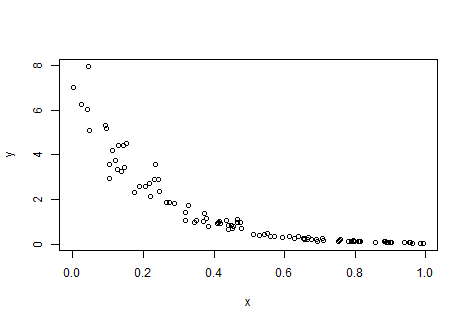
\includegraphics[width=0.7\linewidth]{images/grafico-1} 

}

\caption{Gráfico dos dados gerados}\label{fig:grafico}
\end{figure}

\subsubsection{Gráfico da variável
transformada}\label{grafico-da-variavel-transformada}

\begin{Shaded}
\begin{Highlighting}[]
\KeywordTok{plot}\NormalTok{(x, }\KeywordTok{log}\NormalTok{(y), }\DataTypeTok{pch =} \DecValTok{16}\NormalTok{, }\DataTypeTok{cex =} \FloatTok{0.5}\NormalTok{) }
\KeywordTok{abline}\NormalTok{(}\KeywordTok{lm}\NormalTok{(}\KeywordTok{log}\NormalTok{(y) }\OperatorTok{~}\StringTok{ }\NormalTok{x), }\DataTypeTok{col =} \DecValTok{2}\NormalTok{)}
\end{Highlighting}
\end{Shaded}

\begin{figure}[H]

{\centering 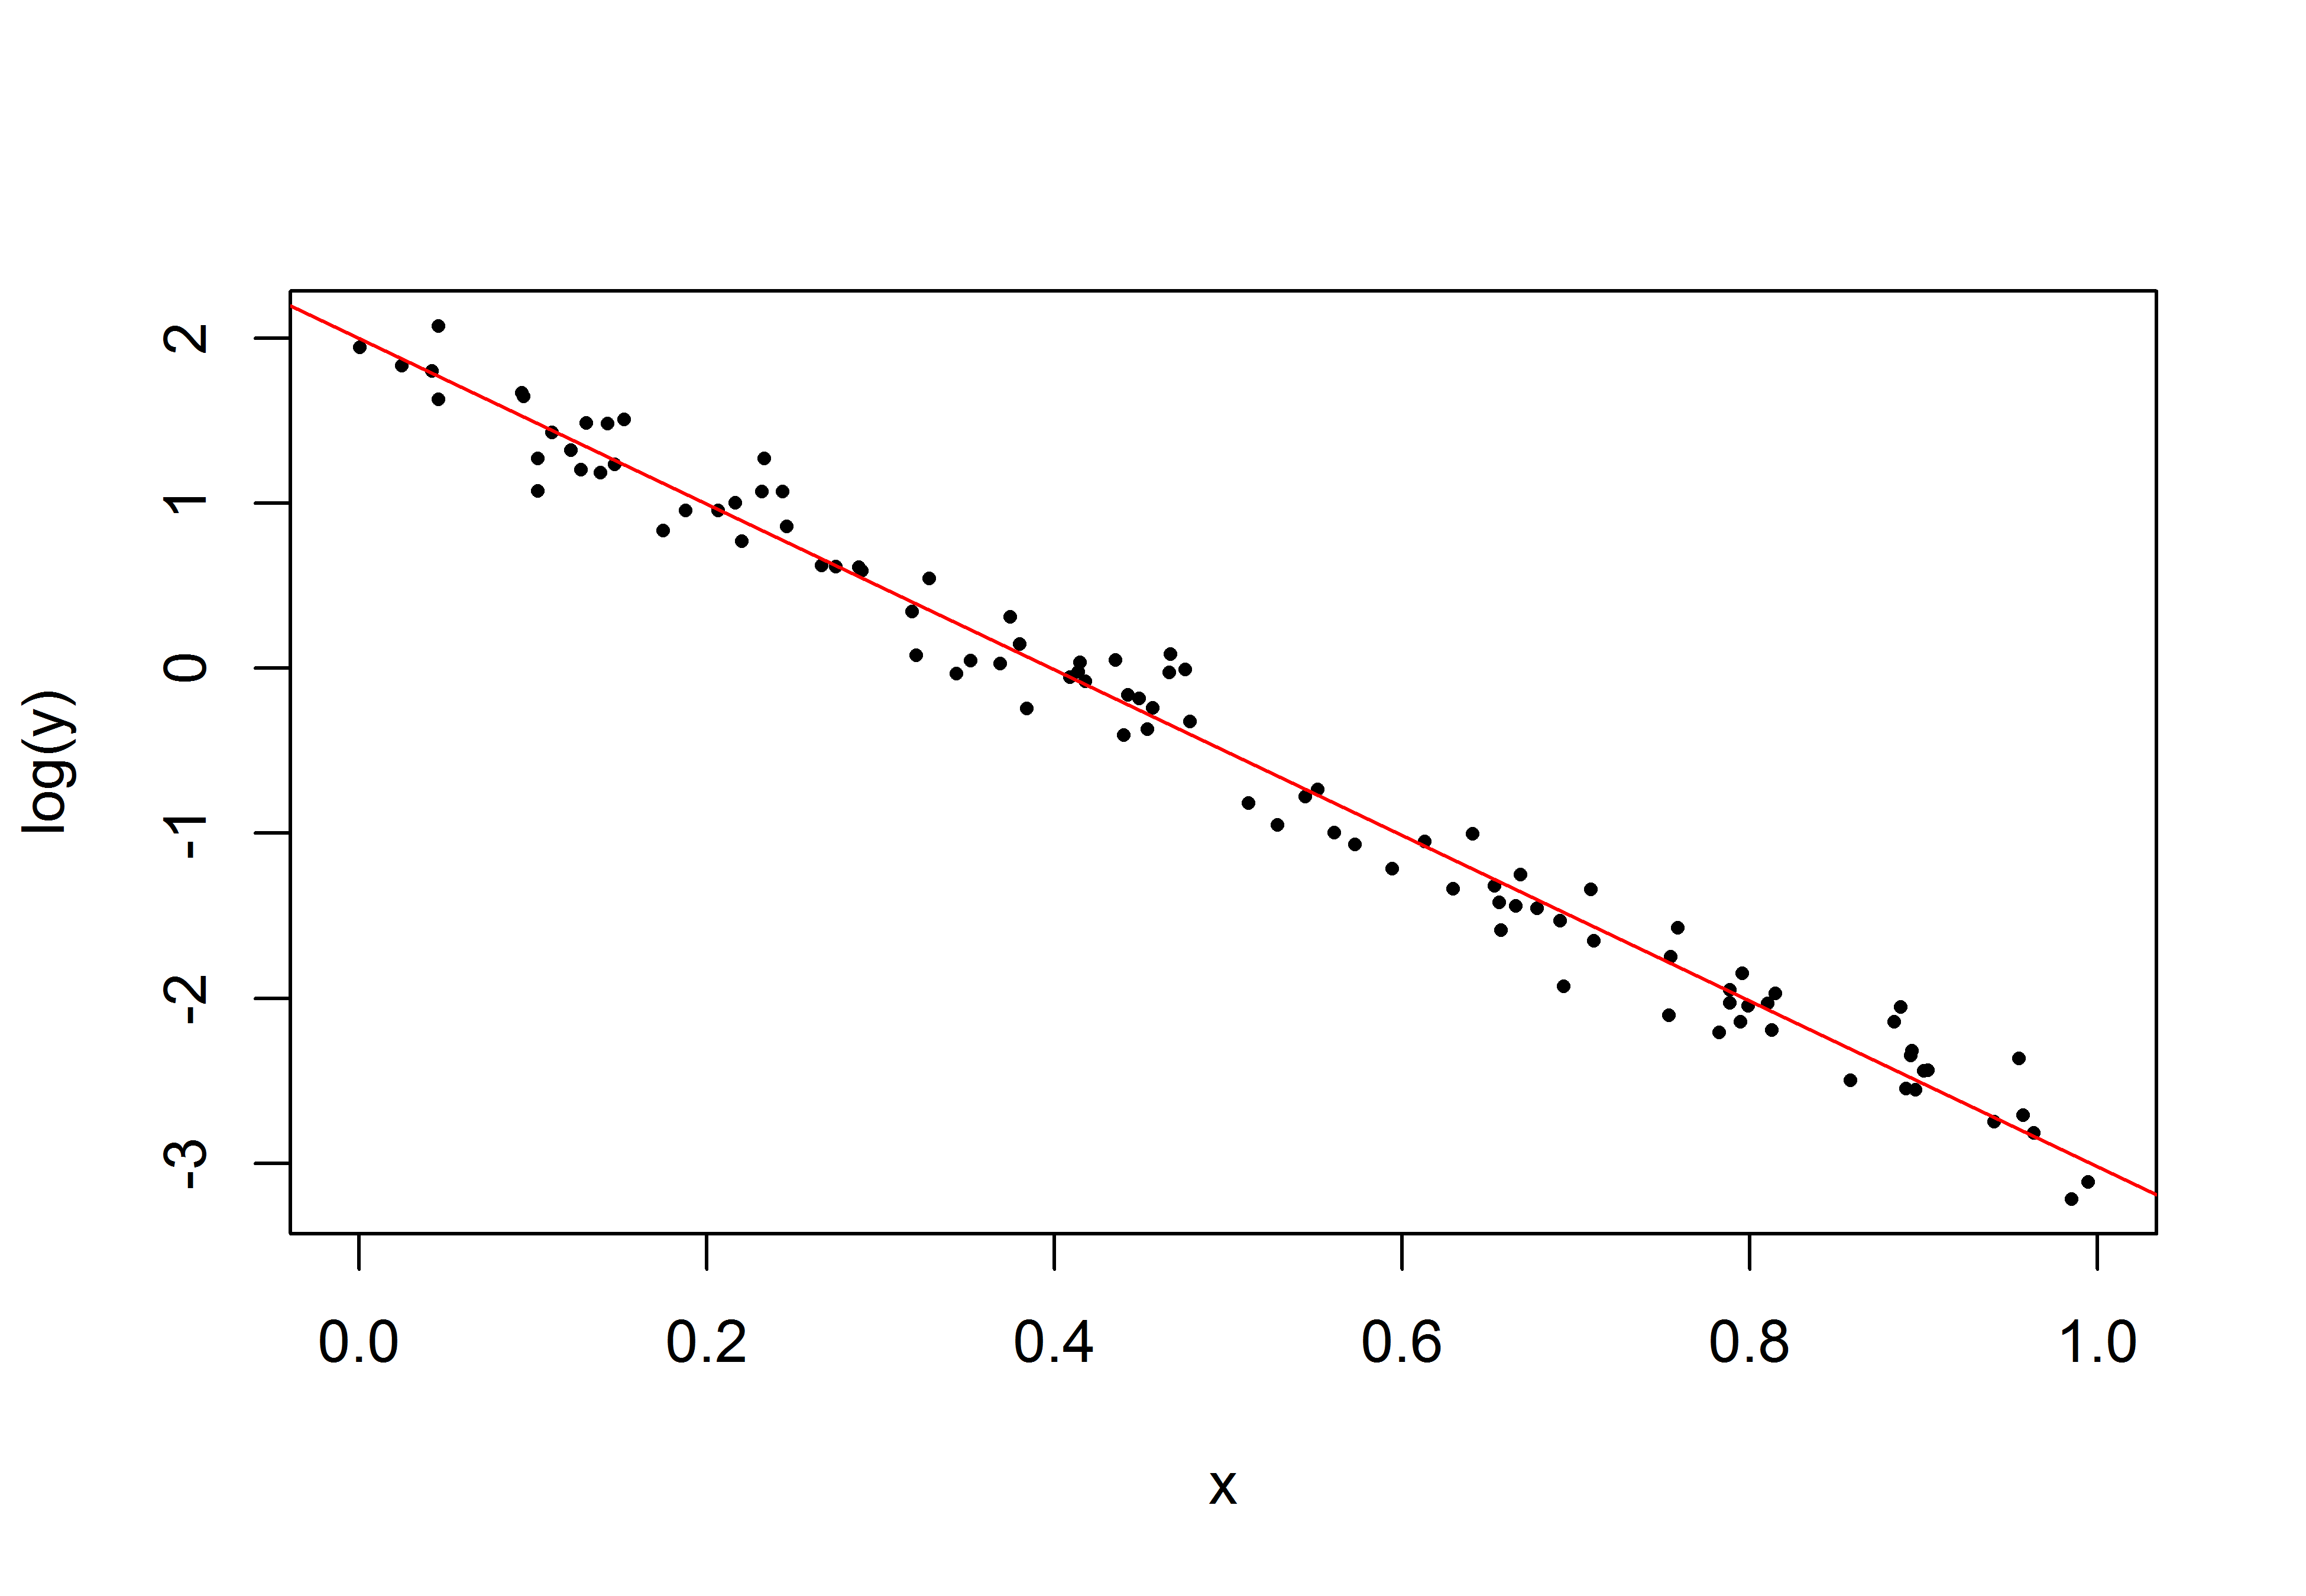
\includegraphics[width=0.7\linewidth]{images/graficotrans-1} 

}

\caption{Gráfico da variável transformada}\label{fig:graficotrans}
\end{figure}

\subsection{Ajuste da regressão
não-linear}\label{ajuste-da-regressao-nao-linear}

\begin{Shaded}
\begin{Highlighting}[]
\NormalTok{### NLS Fit}
\NormalTok{NLfit <-}\StringTok{ }\KeywordTok{nls}\NormalTok{(y }\OperatorTok{~}\StringTok{ }\KeywordTok{exp}\NormalTok{(a}\OperatorTok{*}\NormalTok{x}\OperatorTok{+}\NormalTok{b), }\DataTypeTok{start =} \KeywordTok{c}\NormalTok{(}\DataTypeTok{a =} \OperatorTok{-}\DecValTok{10}\NormalTok{, }\DataTypeTok{b =} \DecValTok{15}\NormalTok{)) }
\end{Highlighting}
\end{Shaded}

\subsubsection{Coeficientes}\label{coeficientes}

\begin{Shaded}
\begin{Highlighting}[]
\NormalTok{co <-}\StringTok{ }\KeywordTok{coef}\NormalTok{(NLfit)}
\NormalTok{co}
\end{Highlighting}
\end{Shaded}

\begin{verbatim}
##            a            b 
## -4.896555212  1.997874467
\end{verbatim}

\subsubsection{Gráfico do modelo
não-linear}\label{grafico-do-modelo-nao-linear}

\begin{Shaded}
\begin{Highlighting}[]
\NormalTok{f <-}\StringTok{ }\ControlFlowTok{function}\NormalTok{(x,a,b) \{}\KeywordTok{exp}\NormalTok{(a}\OperatorTok{*}\NormalTok{x}\OperatorTok{+}\NormalTok{b)\}}
\KeywordTok{curve}\NormalTok{(}\KeywordTok{f}\NormalTok{(}\DataTypeTok{x =}\NormalTok{ x, }\DataTypeTok{a =}\NormalTok{ co[}\DecValTok{1}\NormalTok{], }\DataTypeTok{b =}\NormalTok{ co[}\DecValTok{2}\NormalTok{]), }\DataTypeTok{col =} \DecValTok{2}\NormalTok{, }\DataTypeTok{lwd =} \FloatTok{1.2}\NormalTok{) }
\KeywordTok{curve}\NormalTok{(}\KeywordTok{f}\NormalTok{(}\DataTypeTok{x =}\NormalTok{ x, }\DataTypeTok{a =} \OperatorTok{-}\DecValTok{5}\NormalTok{, }\DataTypeTok{b =} \DecValTok{2}\NormalTok{), }\DataTypeTok{col =} \DecValTok{3}\NormalTok{, }\DataTypeTok{lwd =} \FloatTok{1.5}\NormalTok{, }\DataTypeTok{add =} \OtherTok{TRUE}\NormalTok{)}
\end{Highlighting}
\end{Shaded}

\begin{figure}[H]

{\centering 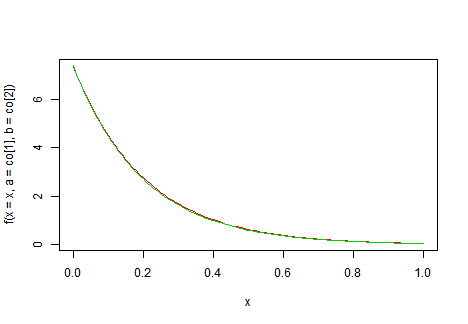
\includegraphics[width=0.7\linewidth]{images/graficoNL-1} 

}

\caption{Gráfico do modelo não-linear}\label{fig:graficoNL}
\end{figure}

\subsubsection{Estimativas do modelo
não-linear}\label{estimativas-do-modelo-nao-linear}

\begin{Shaded}
\begin{Highlighting}[]
\NormalTok{pNLfit <-}\StringTok{ }\KeywordTok{predict}\NormalTok{(NLfit, }\DataTypeTok{newdata =} \KeywordTok{data.frame}\NormalTok{(}\DataTypeTok{x =}\NormalTok{ .}\DecValTok{7}\NormalTok{))}
\NormalTok{pNLfit}
\end{Highlighting}
\end{Shaded}

\begin{verbatim}
## [1] 0.2393773308
\end{verbatim}

O valor teórico obtido pela equação original (\(y = e^{-5x + 2}\)) é de:

\begin{Shaded}
\begin{Highlighting}[]
\NormalTok{Yteorico <-}\StringTok{ }\KeywordTok{exp}\NormalTok{(}\OperatorTok{-}\DecValTok{5}\OperatorTok{*}\NormalTok{.}\DecValTok{7} \OperatorTok{+}\StringTok{ }\DecValTok{2}\NormalTok{)}
\KeywordTok{round}\NormalTok{(Yteorico, }\DecValTok{4}\NormalTok{)}
\end{Highlighting}
\end{Shaded}

\begin{verbatim}
## [1] 0.2231
\end{verbatim}

\[\epsilon = \frac{\hat{Y} - Y_{teórico}}{Y_{teórico}}\]

O valor obtido pelo modelo é muito próximo do valor teórico. O erro do
modelo, portanto, é de 7.28\%.

\subsection{Ajuste de modelo linear
generalizado}\label{ajuste-de-modelo-linear-generalizado}

\subsubsection{Poisson}\label{poisson}

\begin{Shaded}
\begin{Highlighting}[]
\NormalTok{Gfit <-}\StringTok{ }\KeywordTok{glm}\NormalTok{(y }\OperatorTok{~}\StringTok{ }\NormalTok{x, }\DataTypeTok{family =} \KeywordTok{poisson}\NormalTok{())}
\KeywordTok{summary}\NormalTok{(Gfit)}
\end{Highlighting}
\end{Shaded}

\begin{verbatim}
## 
## Call:
## glm(formula = y ~ x, family = poisson())
## 
## Deviance Residuals: 
##         Min           1Q       Median           3Q          Max  
## -0.78105080  -0.11407910  -0.02334406   0.04517457   0.78120241  
## 
## Coefficients:
##               Estimate Std. Error   z value   Pr(>|z|)    
## (Intercept)  2.0129853  0.1265714  15.90394 < 2.22e-16 ***
## x           -4.9957447  0.4647721 -10.74881 < 2.22e-16 ***
## ---
## Signif. codes:  0 '***' 0.001 '**' 0.01 '*' 0.05 '.' 0.1 ' ' 1
## 
## (Dispersion parameter for poisson family taken to be 1)
## 
##     Null deviance: 184.288851  on 99  degrees of freedom
## Residual deviance:   4.991623  on 98  degrees of freedom
## AIC: Inf
## 
## Number of Fisher Scoring iterations: 4
\end{verbatim}

\paragraph{Estimativa com o modelo linear generalizado com
Poisson}\label{estimativa-com-o-modelo-linear-generalizado-com-poisson}

\begin{Shaded}
\begin{Highlighting}[]
\NormalTok{pGfit <-}\StringTok{ }\KeywordTok{predict}\NormalTok{(Gfit, }\DataTypeTok{newdata =} \KeywordTok{data.frame}\NormalTok{(}\DataTypeTok{x =}\NormalTok{ .}\DecValTok{7}\NormalTok{), }\DataTypeTok{type =} \StringTok{"response"}\NormalTok{)}
\NormalTok{pGfit}
\end{Highlighting}
\end{Shaded}

\begin{verbatim}
##            1 
## 0.2267207901
\end{verbatim}

O valor obtido pelo modelo também é muito próximo do valor teórico
obtido pela equação original (\(y = e^{-5x + 2}\)). Neste caso, o erro
do modelo é de 1.61\%.

\subsubsection{Gauss}\label{gauss}

\begin{Shaded}
\begin{Highlighting}[]
\NormalTok{Gfit2 <-}\StringTok{ }\KeywordTok{glm}\NormalTok{(y }\OperatorTok{~}\StringTok{ }\NormalTok{x, }\DataTypeTok{family =} \KeywordTok{gaussian}\NormalTok{(}\DataTypeTok{link =} \StringTok{"log"}\NormalTok{))}
\KeywordTok{summary}\NormalTok{(Gfit2)}
\end{Highlighting}
\end{Shaded}

\begin{verbatim}
## 
## Call:
## glm(formula = y ~ x, family = gaussian(link = "log"))
## 
## Deviance Residuals: 
##         Min           1Q       Median           3Q          Max  
## -1.52566206  -0.10270628  -0.01630332   0.02118162   2.06949483  
## 
## Coefficients:
##               Estimate Std. Error   t value   Pr(>|t|)    
## (Intercept)  1.9978743  0.0268358  74.44810 < 2.22e-16 ***
## x           -4.8965539  0.1736556 -28.19692 < 2.22e-16 ***
## ---
## Signif. codes:  0 '***' 0.001 '**' 0.01 '*' 0.05 '.' 0.1 ' ' 1
## 
## (Dispersion parameter for gaussian family taken to be 0.1633725569)
## 
##     Null deviance: 313.906827  on 99  degrees of freedom
## Residual deviance:  16.010526  on 98  degrees of freedom
## AIC: 106.59533
## 
## Number of Fisher Scoring iterations: 4
\end{verbatim}

\paragraph{Estimativa com o modelo linear generalizado com
Gauss}\label{estimativa-com-o-modelo-linear-generalizado-com-gauss}

\begin{Shaded}
\begin{Highlighting}[]
\NormalTok{pGfit2 <-}\StringTok{ }\KeywordTok{predict}\NormalTok{(Gfit2, }\DataTypeTok{newdata =} \KeywordTok{data.frame}\NormalTok{(}\DataTypeTok{x =}\NormalTok{ .}\DecValTok{7}\NormalTok{), }\DataTypeTok{type =} \StringTok{"response"}\NormalTok{)}
\NormalTok{pGfit2}
\end{Highlighting}
\end{Shaded}

\begin{verbatim}
##            1 
## 0.2393775107
\end{verbatim}

O valor obtido pelo modelo também é muito próximo do valor teórico
obtido pela equação original (\(y = e^{-5x + 2}\)). Neste caso, o erro
do modelo é de 7.28\%. Observar que a adoção de ajuste por modelo linear
generalizado com família gaussiana e \emph{log-link} é equivalente ao
ajustamento de um modelo de regressão não-linear, como visto na seção
anterior.

\subsection{Ajuste de Regressão Linear com variável dependente
transformada}\label{ajuste-de-regressao-linear-com-variavel-dependente-transformada}

\begin{Shaded}
\begin{Highlighting}[]
\NormalTok{### LM Fit}
\NormalTok{fit <-}\StringTok{ }\KeywordTok{lm}\NormalTok{(}\KeywordTok{log}\NormalTok{(y) }\OperatorTok{~}\StringTok{ }\NormalTok{x)}
\NormalTok{s <-}\StringTok{ }\KeywordTok{summary}\NormalTok{(fit)}
\NormalTok{s}
\end{Highlighting}
\end{Shaded}

\begin{verbatim}
## 
## Call:
## lm(formula = log(y) ~ x)
## 
## Residuals:
##         Min          1Q      Median          3Q         Max 
## -0.44759471 -0.12264594 -0.00394687  0.11926677  0.44344532 
## 
## Coefficients:
##                Estimate  Std. Error   t value   Pr(>|t|)    
## (Intercept)  1.99820803  0.03921100  50.96040 < 2.22e-16 ***
## x           -5.01796627  0.06836424 -73.40045 < 2.22e-16 ***
## ---
## Signif. codes:  0 '***' 0.001 '**' 0.01 '*' 0.05 '.' 0.1 ' ' 1
## 
## Residual standard error: 0.1938582 on 98 degrees of freedom
## Multiple R-squared:  0.9821351,  Adjusted R-squared:  0.9819528 
## F-statistic: 5387.626 on 1 and 98 DF,  p-value: < 2.2204e-16
\end{verbatim}

\subsubsection{Gráfico do modelo linear}\label{grafico-do-modelo-linear}

\begin{Shaded}
\begin{Highlighting}[]
\CommentTok{#plotmod(fit)}
\end{Highlighting}
\end{Shaded}

\subsubsection{Estimativas}\label{estimativas}

\begin{enumerate}
\def\labelenumi{\alph{enumi}.}
\tightlist
\item
  Pela mediana
\end{enumerate}

\begin{Shaded}
\begin{Highlighting}[]
\NormalTok{Y <-}\StringTok{ }\KeywordTok{predict}\NormalTok{(fit, }\DataTypeTok{newdata =} \KeywordTok{data.frame}\NormalTok{(}\DataTypeTok{x =}\NormalTok{ .}\DecValTok{7}\NormalTok{))}
\NormalTok{p_mediana <-}\StringTok{ }\KeywordTok{exp}\NormalTok{(Y)}
\NormalTok{p_mediana}
\end{Highlighting}
\end{Shaded}

\begin{verbatim}
##            1 
## 0.2199470683
\end{verbatim}

O erro do modelo, neste caso, é de -1.43\%.

\begin{enumerate}
\def\labelenumi{\alph{enumi}.}
\setcounter{enumi}{1}
\tightlist
\item
  Pela moda
\end{enumerate}

\begin{Shaded}
\begin{Highlighting}[]
\NormalTok{p_moda <-}\StringTok{ }\KeywordTok{exp}\NormalTok{(Y }\OperatorTok{-}\StringTok{ }\NormalTok{s}\OperatorTok{$}\NormalTok{sigma}\OperatorTok{^}\DecValTok{2}\NormalTok{)}
\NormalTok{p_moda}
\end{Highlighting}
\end{Shaded}

\begin{verbatim}
##            1 
## 0.2118346261
\end{verbatim}

O erro do modelo, neste caso, é de -5.06\%.

\begin{enumerate}
\def\labelenumi{\alph{enumi}.}
\setcounter{enumi}{2}
\tightlist
\item
  Pela média
\end{enumerate}

\begin{Shaded}
\begin{Highlighting}[]
\NormalTok{p_media <-}\StringTok{ }\KeywordTok{exp}\NormalTok{(Y }\OperatorTok{+}\StringTok{ }\NormalTok{s}\OperatorTok{$}\NormalTok{sigma}\OperatorTok{^}\DecValTok{2}\OperatorTok{/}\DecValTok{2}\NormalTok{)}
\NormalTok{p_media}
\end{Highlighting}
\end{Shaded}

\begin{verbatim}
##            1 
## 0.2241190594
\end{verbatim}

O erro do modelo, neste caso, é de 0.443\%.

\subsection{Comparação dos resultados
obtidos}\label{comparacao-dos-resultados-obtidos}

\begin{longtable}[]{@{}lrr@{}}
\toprule
Modelo & Previsão & Erro (\%)\tabularnewline
\midrule
\endhead
\textbf{Valor Teórico} & \textbf{0.2231} & ------\tabularnewline
Regressão Não-Linear & 0.2394 & 7.28\%\tabularnewline
GLM (Poisson) & 0.2267 & 1.61\%\tabularnewline
GLM (Gauss) & 0.2394 & 7.28\%\tabularnewline
LM (Mediana) & 0.2199 & -1.43\%\tabularnewline
LM (Moda) & 0.2118 & -5.06\%\tabularnewline
LM (Média) & 0.2241 & 0.443\%\tabularnewline
\bottomrule
\end{longtable}

\section{Método de Monte-Carlo}\label{metodo-de-monte-carlo}

O resultados acima não devem ser interpretados como taxativos, pois os
valores encontrados foram obtidos de dados gerados randômicamente.

Para uma comparação mais precisa entre os modelos testados, utilizamos o
método de Monte Carlo, simulando os dados randomicamente a cada
iteração. Finalmente, comparamos o valor médio obtido por cada cada
modelo ao valor téorico.

\begin{Shaded}
\begin{Highlighting}[]
\NormalTok{Nsim <-}\StringTok{ }\DecValTok{500}
\NormalTok{pNL <-}\StringTok{ }\KeywordTok{vector}\NormalTok{(}\DataTypeTok{mode =} \StringTok{"numeric"}\NormalTok{, }\DataTypeTok{length =}\NormalTok{ Nsim)}
\NormalTok{pG <-}\StringTok{ }\KeywordTok{vector}\NormalTok{(}\DataTypeTok{mode =} \StringTok{"numeric"}\NormalTok{, }\DataTypeTok{length =}\NormalTok{ Nsim)}
\NormalTok{pG2 <-}\StringTok{ }\KeywordTok{vector}\NormalTok{(}\DataTypeTok{mode =} \StringTok{"numeric"}\NormalTok{, }\DataTypeTok{length =}\NormalTok{ Nsim)}
\NormalTok{p_mediana <-}\StringTok{ }\KeywordTok{vector}\NormalTok{(}\DataTypeTok{mode =} \StringTok{"numeric"}\NormalTok{, }\DataTypeTok{length =}\NormalTok{ Nsim)}
\NormalTok{p_moda <-}\StringTok{ }\KeywordTok{vector}\NormalTok{(}\DataTypeTok{mode =} \StringTok{"numeric"}\NormalTok{, }\DataTypeTok{length =}\NormalTok{ Nsim)}
\NormalTok{p_media <-}\StringTok{ }\KeywordTok{vector}\NormalTok{(}\DataTypeTok{mode =} \StringTok{"numeric"}\NormalTok{, }\DataTypeTok{length =}\NormalTok{ Nsim)}
\ControlFlowTok{for}\NormalTok{ (i }\ControlFlowTok{in} \DecValTok{1}\OperatorTok{:}\NormalTok{Nsim) \{}
\NormalTok{  y =}\StringTok{ }\KeywordTok{exp}\NormalTok{(a}\OperatorTok{*}\NormalTok{x }\OperatorTok{+}\StringTok{ }\NormalTok{b }\OperatorTok{+}\StringTok{ }\KeywordTok{rnorm}\NormalTok{(}\DecValTok{100}\NormalTok{, }\DecValTok{0}\NormalTok{, .}\DecValTok{2}\NormalTok{))}
\NormalTok{  NLfit <-}\StringTok{ }\KeywordTok{nls}\NormalTok{(y }\OperatorTok{~}\StringTok{ }\KeywordTok{exp}\NormalTok{(a}\OperatorTok{*}\NormalTok{x}\OperatorTok{+}\NormalTok{b), }\DataTypeTok{start =} \KeywordTok{c}\NormalTok{(}\DataTypeTok{a =} \OperatorTok{-}\DecValTok{10}\NormalTok{, }\DataTypeTok{b =} \DecValTok{15}\NormalTok{)) }
\NormalTok{  Gfit <-}\StringTok{ }\KeywordTok{glm}\NormalTok{(y }\OperatorTok{~}\StringTok{ }\NormalTok{x, }\DataTypeTok{family =} \KeywordTok{poisson}\NormalTok{())}
\NormalTok{  Gfit2 <-}\StringTok{ }\KeywordTok{glm}\NormalTok{(y }\OperatorTok{~}\StringTok{ }\NormalTok{x, }\DataTypeTok{family =} \KeywordTok{gaussian}\NormalTok{(}\DataTypeTok{link =} \StringTok{"log"}\NormalTok{))}
\NormalTok{  fit <-}\StringTok{ }\KeywordTok{lm}\NormalTok{(}\KeywordTok{log}\NormalTok{(y) }\OperatorTok{~}\StringTok{ }\NormalTok{x)}
\NormalTok{  s <-}\StringTok{ }\KeywordTok{summary}\NormalTok{(fit)}
\NormalTok{  pNL[i] <-}\StringTok{ }\KeywordTok{predict}\NormalTok{(NLfit, }\DataTypeTok{newdata =} \KeywordTok{data.frame}\NormalTok{(}\DataTypeTok{x =}\NormalTok{ .}\DecValTok{7}\NormalTok{))}
\NormalTok{  pG[i] <-}\StringTok{ }\KeywordTok{predict}\NormalTok{(Gfit, }\DataTypeTok{newdata =} \KeywordTok{data.frame}\NormalTok{(}\DataTypeTok{x =}\NormalTok{ .}\DecValTok{7}\NormalTok{), }\DataTypeTok{type =} \StringTok{"response"}\NormalTok{)}
\NormalTok{  pG2[i] <-}\StringTok{ }\KeywordTok{predict}\NormalTok{(Gfit2, }\DataTypeTok{newdata =} \KeywordTok{data.frame}\NormalTok{(}\DataTypeTok{x =}\NormalTok{ .}\DecValTok{7}\NormalTok{), }\DataTypeTok{type =} \StringTok{"response"}\NormalTok{)}
\NormalTok{  p_mediana[i] <-}\StringTok{ }\KeywordTok{exp}\NormalTok{(}\KeywordTok{predict}\NormalTok{(fit, }\DataTypeTok{newdata =} \KeywordTok{data.frame}\NormalTok{(}\DataTypeTok{x =}\NormalTok{ .}\DecValTok{7}\NormalTok{)))}
\NormalTok{  p_moda[i] <-}\StringTok{ }\KeywordTok{exp}\NormalTok{(}\KeywordTok{predict}\NormalTok{(fit, }\DataTypeTok{newdata =} \KeywordTok{data.frame}\NormalTok{(}\DataTypeTok{x =}\NormalTok{ .}\DecValTok{7}\NormalTok{)) }\OperatorTok{-}\StringTok{ }\NormalTok{s}\OperatorTok{$}\NormalTok{sigma}\OperatorTok{^}\DecValTok{2}\NormalTok{)}
\NormalTok{  p_media[i] <-}\StringTok{ }\KeywordTok{exp}\NormalTok{(}\KeywordTok{predict}\NormalTok{(fit, }\DataTypeTok{newdata =} \KeywordTok{data.frame}\NormalTok{(}\DataTypeTok{x =}\NormalTok{ .}\DecValTok{7}\NormalTok{)) }\OperatorTok{+}\StringTok{ }\NormalTok{s}\OperatorTok{$}\NormalTok{sigma}\OperatorTok{^}\DecValTok{2}\OperatorTok{/}\DecValTok{2}\NormalTok{)}
\NormalTok{\}}
\end{Highlighting}
\end{Shaded}

\begin{itemize}
\tightlist
\item
  Gráficos
\end{itemize}

\begin{figure}[H]

{\centering 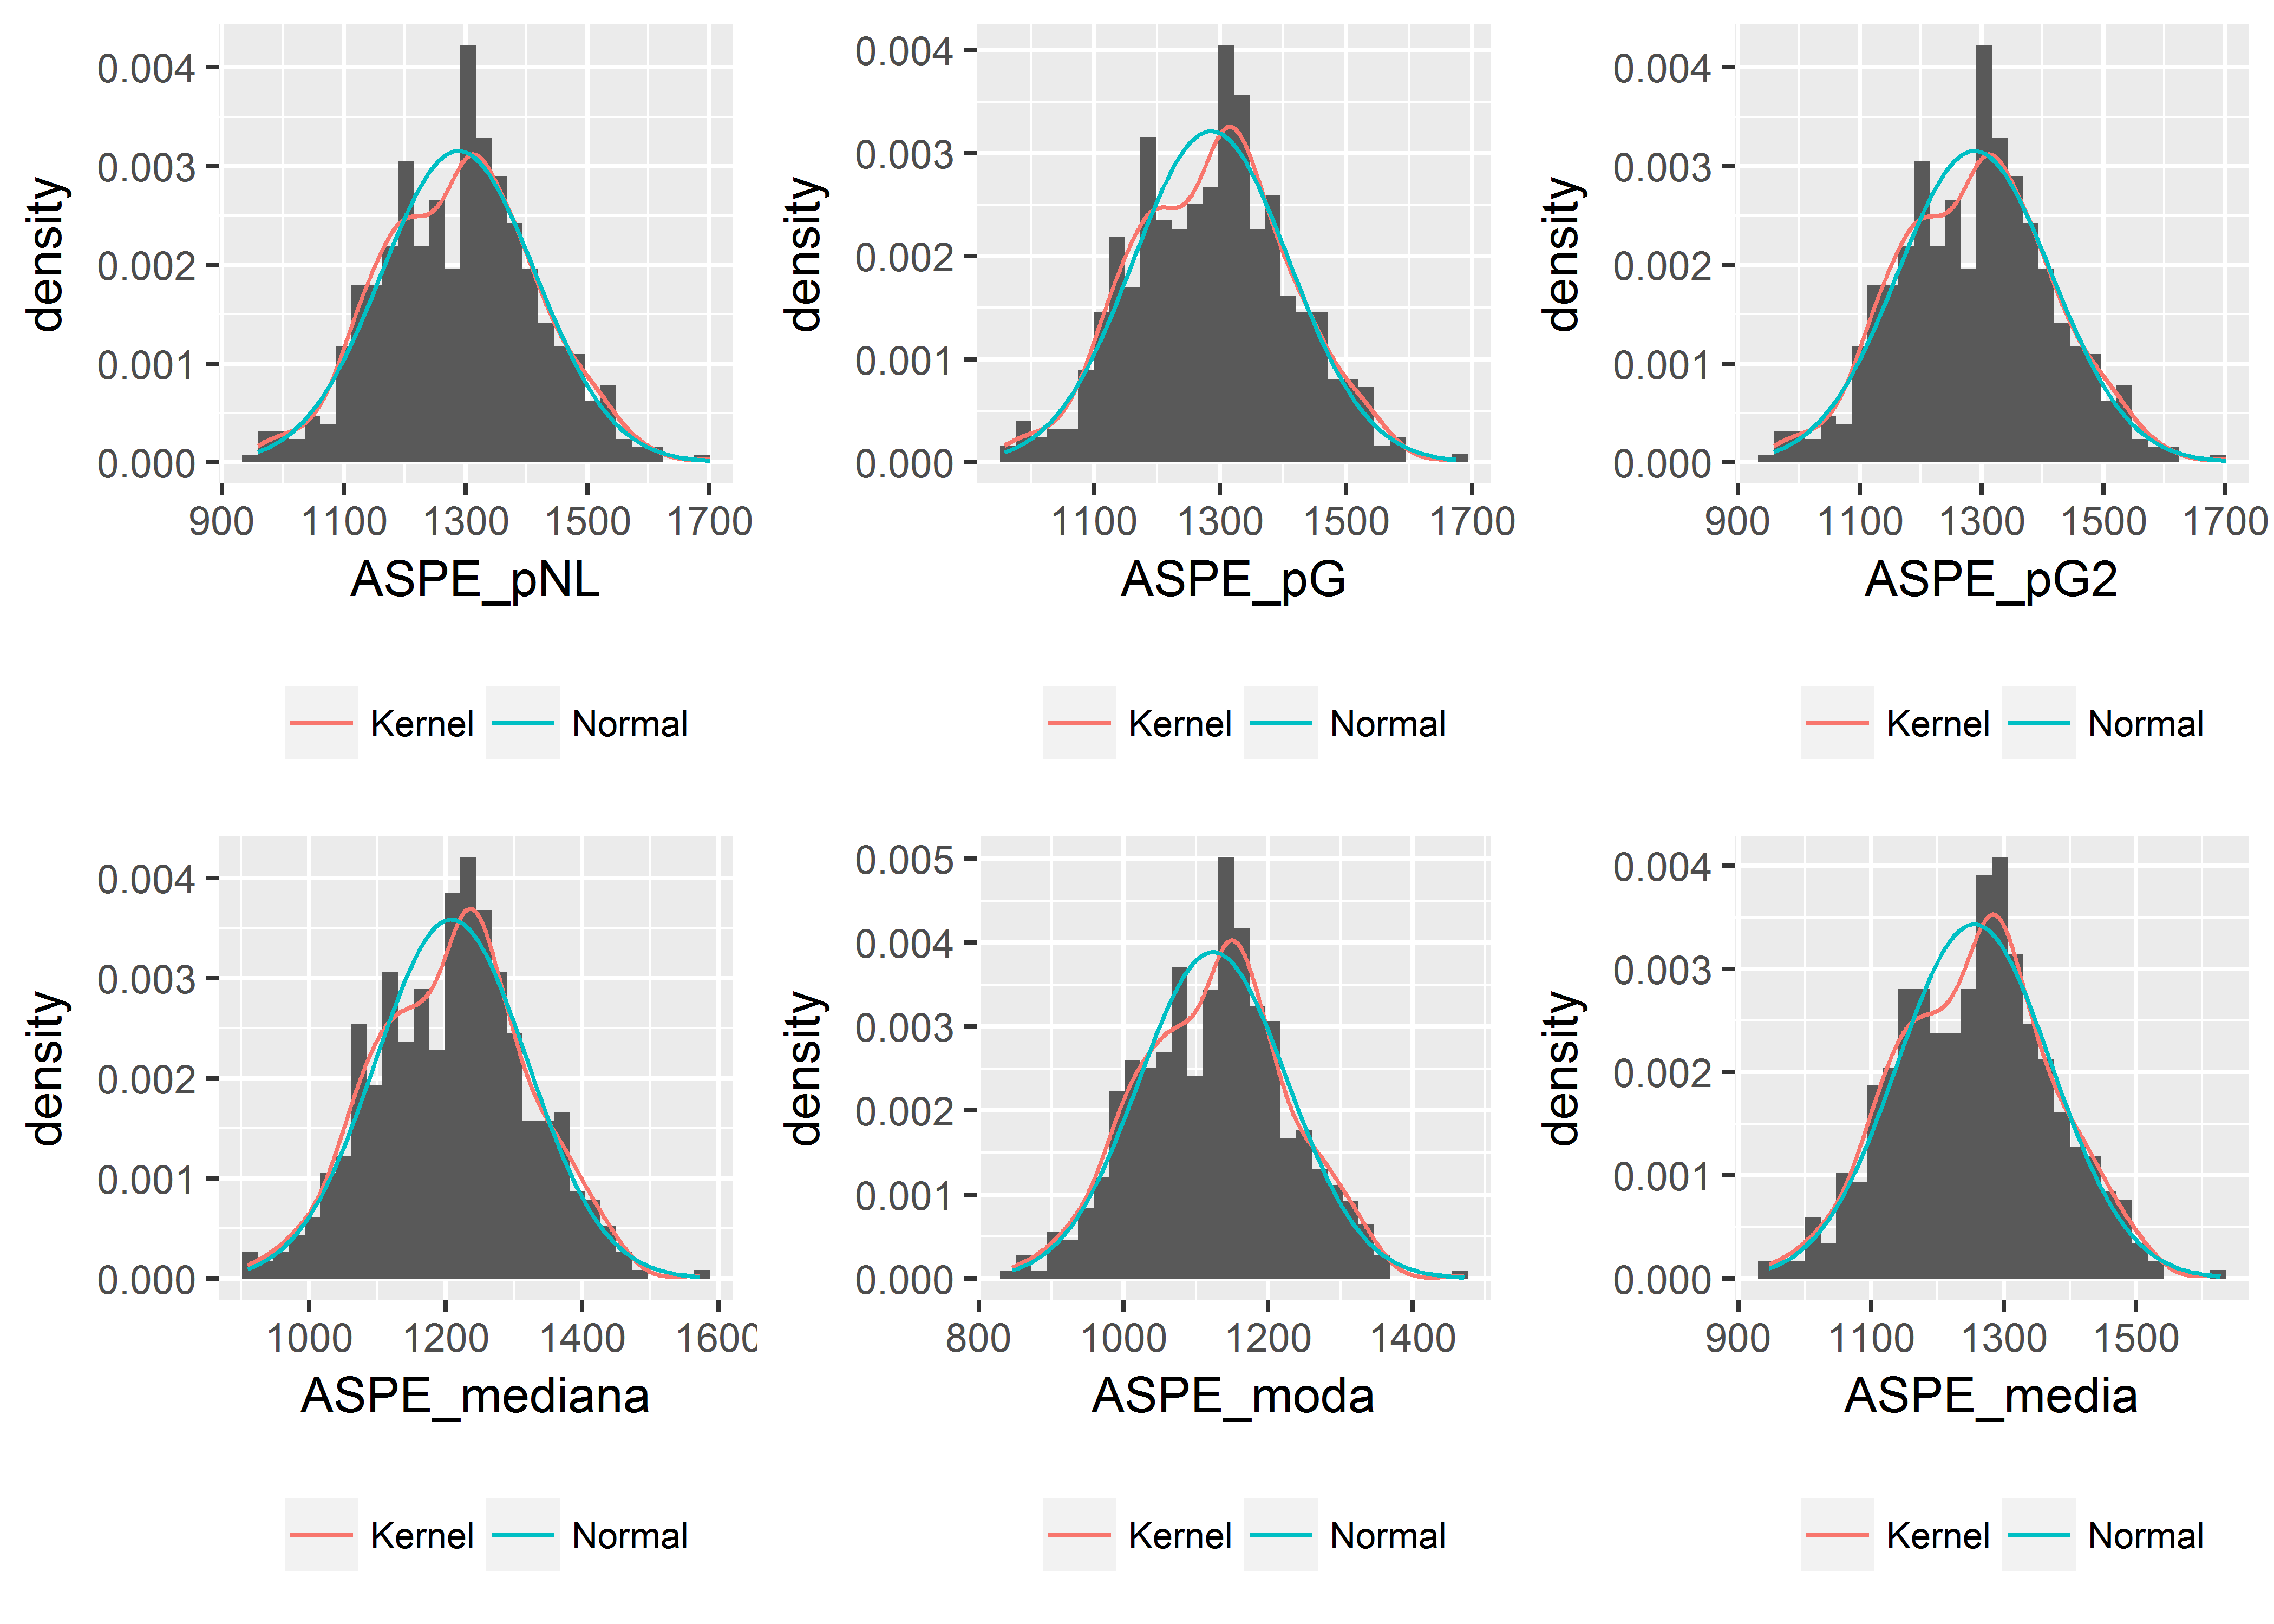
\includegraphics[width=1\linewidth]{images/histogramas-1} 

}

\caption{Histogramas das variáveis simuladas}\label{fig:histogramas}
\end{figure}

\begin{longtable}[]{@{}lrrr@{}}
\toprule
Modelo & Previsão & \(\sigma^2\) & Erro\tabularnewline
\midrule
\endhead
\textbf{Valor Teórico} & \textbf{0.2231} & ------ &
------\tabularnewline
Regressão Não-Linear & 0.2275 & 0.0389 & 1.96\%\tabularnewline
GLM (Poisson) & 0.2279 & 0.0111 & 2.16\%\tabularnewline
GLM (Gauss) & 0.2275 & 0.0389 & 1.96\%\tabularnewline
LM (Mediana) & 0.2236 & 0.0052 & 0.207\%\tabularnewline
LM (Moda) & 0.2148 & 0.0052 & -3.72\%\tabularnewline
LM (Média) & 0.2281 & 0.0053 & 2.23\%\tabularnewline
\bottomrule
\end{longtable}

\section*{REFERÊNCIAS}\label{referencias}
\addcontentsline{toc}{section}{REFERÊNCIAS}

\hypertarget{refs}{}
\hypertarget{ref-Duan}{}
DUAN, N. Smearing estimate: A nonparametric retransformation method.
\textbf{Journal of the American Statistical Association}, v. 78, n. 383,
p. 605--610, 1983. Taylor \& Francis. Disponível em:
\textless{}\url{http://www.tandfonline.com/doi/abs/10.1080/01621459.1983.10478017}\textgreater{}..

\hypertarget{ref-NBERt0246}{}
MANNING, W. G.; MULLAHY, J. \textbf{Estimating log models: To transform
or not to transform?} Working Paper, National Bureau of Economic
Research, 1999.

\hypertarget{ref-wiki:E}{}
WIKIPEDIA. Valor esperado --- Wikipedia, the free encyclopedia., 2018.
Disponível em:
\textless{}\url{https://pt.wikipedia.org/wiki/Valor_esperado}\textgreater{}..


\end{document}
